\documentclass{ximera}

\title{Increasing and Decreasing Functions Activity Facilitator Guide}
\author{MATH 425: Calculus I}

\begin{document}
\begin{abstract}
   Working with the peers in your group, solve the following problems. Make sure to show and justify all your work. Make sure everyone in the group understands the solution and participates. Be prepared to report your answers to the whole class. 
\end{abstract}
\maketitle

\textbf{Student Learning Objectives}\\
Students should be able to: 
    \begin{itemize}
        \item Find critical points for functions.
        \item Use sign diagrams to find intervals of increasing and decreasing. 
        \item Find intervals of increasing and decreasing based on the graph of a derivative. 
        \item Draw conclusions about the shape of a function from intervals of increasing and decreasing and derivative information.
    \end{itemize}

\textbf{Prerequisites:} Students are expected to know how to find critical numbers of functions and use them to set up a sign diagram.  Problems 3 and 4 ask students to go further and interepret shape of the function based on the derivative.  These will be the more challenging problems, as students may not have thought through the implications of the derivative in this way before.\\

This worksheet may be a bit on the shorter side, especially if students move quickly through (3) and (4).  

\begin{exercise}
    Find all intervals of increasing and decreasing for the function $f(x)=3x^5-5x^3$.  Identify any local extrema.\\
    \textcolor{blue}{$f'(x)=15x^4-15x^2$\\
    $f'(x)=0$ means $15x^2(x^2-1)=0$, so $15x^2=0$ or $x^2-1=0$\\
    This means $x=-1, 0, 1$\\
    $f'$ exists everywhere, since it is a polynomial.\\
    Critical numbers: $x=-1,0,1$\\
    Test points:\\
    For $(-\infty,-1)$: $f'(-2)=15(-2)^4-15(-2)^2=180>0$\\
    For $(-1,0)$: $f'(-\frac12)=15(-\frac12)^4-15(-\frac12)^2=-2.8125<0$\\
    For $(0,1)$: $f'(\frac12)=15(\frac12)^4-15(\frac12)^2=-2.8125<0$\\
    For $(1,\infty)$: $f'(2)=15(2)^4-15(2)^2=180>0$\\
    $f(x)$ is increasing on $(-\infty,-1)$ and $(1,\infty)$\\
    decreasing on $(-1,0)$, $(0,1)$}
\end{exercise}

\begin{exercise}
    Let $h(x)=\frac{1}{3}x^3-5x^2+24x+2$. Find the intervals of increase and decrease for $h$ and identify any local extrema.\\
    \textcolor{blue}{$h'(x)=x^2-10x+24$\\
    $h'(x)=0$ means $x^2-10x+24=0$\\
    This factors as $(x-4)(x-6)=0$, so $x=4$ or $x=6$\\
    $h'$ exists everywhere, since it is a polynomial.\\
    Critical numbers: $x=4,6$\\
    Test points:\\
    For $(-\infty,4)$: $h'(0)=0^2-10(0)+24=24>0$\\
    For $(4,6)$: $h'(5)=5^2-10(5)+24=-1<0$\\
    For $(6,\infty)$: $h'(7)=7^2-10(7)+24=3>0$\\
    $h(x)$ is increasing on $(-\infty,4)$ and $(6,\infty)$\\
    decreasing on $(4,6)$}
\end{exercise}

\begin{exercise}
    Suppose that $g$ is a function whose first derivative is \[g'(x)=\frac{(x+4)(x-2)}{x^2+1}.\]
    \begin{enumerate}
        \item Determine, with justification, all critical numbers of $g$.\\
        \textcolor{blue}{$g'(x)=0$ when $(x+4)(x-2)=0$\\
        so $x=-4, 2$\\
        $g'$ DNE when $x^2+1=0$ which has no solution.\\
        Critical numbers: $x=-4,2$}
        \item  By developing a carefully labeled first derivative sign chart, decide whether $g$ has as a local maximum, local minimum, or neither at each critical number.\\
        \textcolor{blue}{
            \begin{tabular}{c|c|c}
                $(-\infty,-4)$ & $(-4,2)$ & $(2,\infty)$\\
                \hline
                + & - & +\\
            \end{tabular}
        Test points: \\
        $x=-5$: $g'(-5)=\frac{(-5+4)(-5-2)}{(-5)^2+1}=\frac{7}{26}>0$\\
        $x=0$: $g'(0)=\frac{(0+4)(0-2)}{0^2+1}=\frac{-8}{1}<0$\\
        $x=3$: $g'(3)=\frac{(3+4)(3-2)}{3^2+1}=\frac{7}{10}>0$\\
        $g$ has a local min at $x=2$ and a local max at $x=-4$}
        \item Does $g$ have a global maximum? global minimum? Justify your claims.\\
        \textcolor{blue}{Because the function increases, then decreases, then increases, we know that the function will not have any global extrema unless it has a horizontal asymptote. If $\lim_{x\rightarrow -\infty}g(x)$ or $\lim_{x\rightarrow \infty}g(x)$ are not finite, then we know that the function will not have a global max or min, as the values as x gets large in either direction will be either bigger or smaller than what occurs at $x=2$ and $x=-4$. As the end behavior of $g'(x)$ is not approaching 0, we know that $g$ can't have a vertical asymptote.  Thus $g$ has no global max/min. }\\
        \textcolor{orange}{This part will likely not be super familiar for students.  They may just immediately jump to the conclusion that increasing on either end means that the function must have to go towards $\pm \infty$, which is reasonable but lacking the edge case of having a vertical asymptote.  If groups get stuck here, a helpful hint may be to sketch a graph like this and ask them why this situation would not fit the graph you sketched.}
        \item Sketch a possible graph of $y=g(x)$. Clearly label any local or global extrema on the graph.\\
        \begin{center}
            \desmos{tqomxnjqsu}{800}{600}
        \end{center}
        \textcolor{orange}{Students will not need to find the actual equation of the function - they can ignore this part entirely! (This function can be broken down via polynomial division and integrated from there if you want to know how to find this actual equation.)}\\
    Problem from Boelkins, et al., \textit{Active Calculus}, 2nd ed.
    \end{enumerate}
\end{exercise}

\begin{exercise}
    Suppose that $h$ is a differentiable function whose first derivative is given by the graph below.
    \begin{image}
        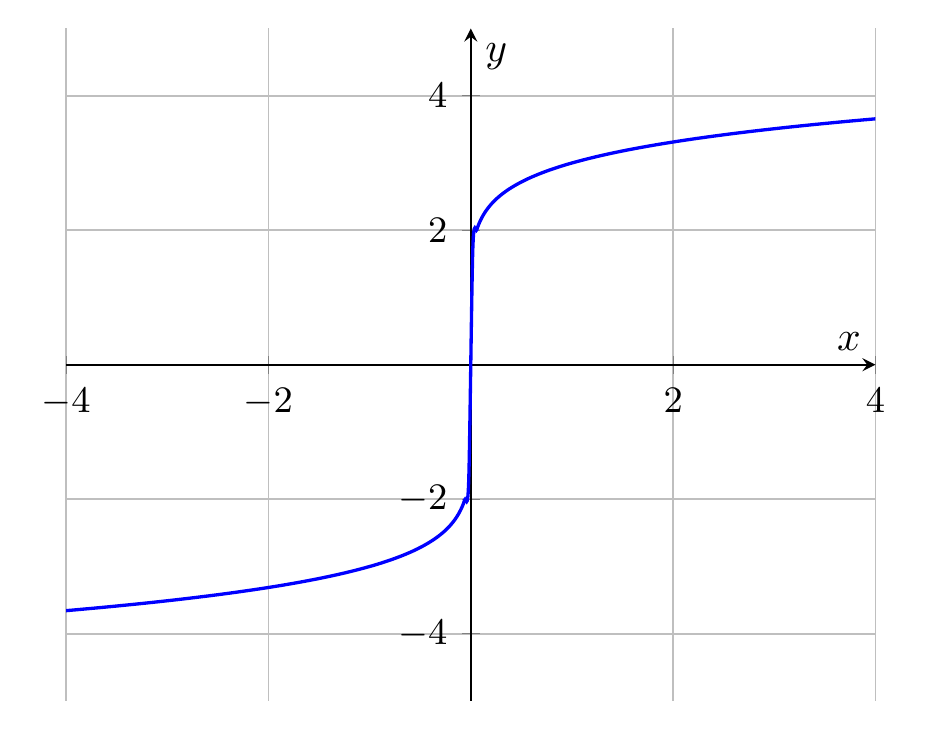
\begin{tikzpicture}[scale=1.5]
            \begin{axis}[
                axis lines=middle,
                xlabel=$x$,
                ylabel=$y$,
                xmin=-4, xmax=4,
                ymin=-5, ymax=5,
                grid=major,
                tick label style={font=\small}
            ]
                \addplot[
                    domain=-4:4,
                    samples=200,
                    smooth,
                    thick,
                    blue
                ] {3*sign(x)*abs(x)^(1/7)};
                %\addlegendentry{$y=3x^{1/9}$}
            \end{axis}
        \end{tikzpicture}  
    \end{image}
    \xmalt{Graph of a function that is negative and increasing before $x=0$, then positive and increasing after $x=0$. }
    \begin{enumerate}
        \item How many real number solutions can $h$ have? Why? \\
        \textcolor{blue}{$h$ can have at most two real solutions, as the function decreases, then increases.  It could cross the $x$ axis once on the decreasing part, then again on the increasing part.  If it does not go low enough to cross the $x$ axis, then it will have 0 solutions.  If the minimum value is on the $x$ axis, then it has one solution.}
        \item If $h(x)$ has two distinct real solutions, what can you say about the signs of the solutions?  Why?\\
        \textcolor{blue}{One solution is before $x=0$ and one solution is after $x=0$, as the function would have to hit once when decreasing ($x<0$) and once when increasing ($x>0$) if there are two solutions.}
        \item Suppose that $\lim_{x\rightarrow \infty}h'(x)=4$, as appears to be indicated by the graph. What can you say about the behavior of $h$ as $x\rightarrow \infty$?  Justify your answer.\\
        \textcolor{blue}{The slope of the tangent lines to the function would approach 4 as the point of tangency $x$ goes toward $\infty$. That would mean the function has to be increasing at a rate of close to 4, so it will be increasing towards $\infty$.}
    \end{enumerate}
\end{exercise}



\end{document}